\documentclass[border=4pt]{standalone}
\usepackage{amsmath,amssymb}
\usepackage{tikz}
\begin{document}
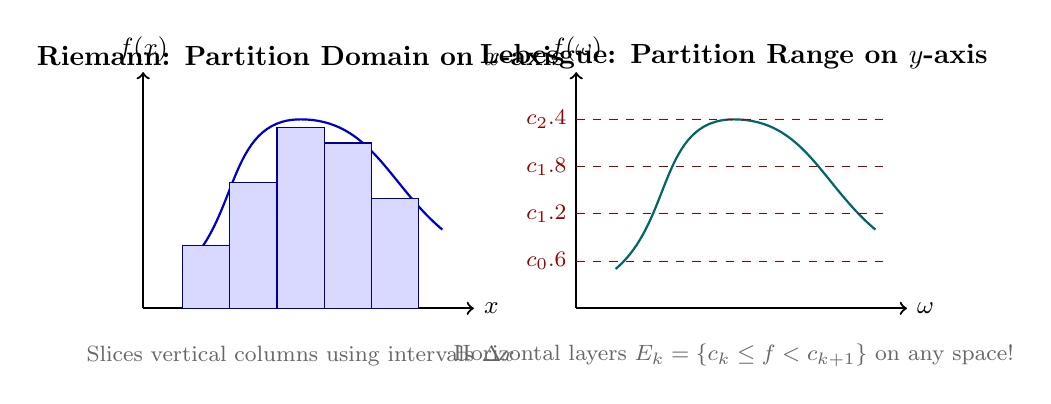
\begin{tikzpicture}[font=\small]
  % Riemann
  \begin{scope}[xshift=0cm]
    \node[font=\bfseries] at (2.0, 3.2) {Riemann: Partition Domain on $x$-axis};
    \draw[->, thick] (0,0) -- (4.2,0) node[right] {$x$};
    \draw[->, thick] (0,0) -- (0,3.0) node[above] {$f(x)$};
    \draw[thick, blue!80!black] (0.5,0.5) to[out=40, in=180] (2.0,2.4) to[out=0, in=140] (3.8,1.0);
    \foreach \x/\h in {0.8/0.8, 1.4/1.6, 2.0/2.3, 2.6/2.1, 3.2/1.4} {
      \draw[fill=blue!15, draw=blue!60!black] (\x-0.3, 0) rectangle (\x+0.3, \h);
    }
    \node[font=\footnotesize, text=gray!80!black] at (2.0, -0.6) {Slices vertical columns using intervals $\Delta x$};
  \end{scope}

  % Lebesgue
  \begin{scope}[xshift=5.5cm]
    \node[font=\bfseries] at (2.0, 3.2) {Lebesgue: Partition Range on $y$-axis};
    \draw[->, thick] (0,0) -- (4.2,0) node[right] {$\omega$};
    \draw[->, thick] (0,0) -- (0,3.0) node[above] {$f(\omega)$};
    \draw[thick, teal!80!black] (0.5,0.5) to[out=40, in=180] (2.0,2.4) to[out=0, in=140] (3.8,1.0);
    \foreach \y in {0.6, 1.2, 1.8, 2.4} {
      \draw[dashed, red!60!black] (0, \y) -- (4.0, \y);
      \node[left, font=\footnotesize, red!60!black] at (0,\y) {$c_\y$};
    }
    \node[font=\footnotesize, text=gray!80!black] at (2.0, -0.6) {Horizontal layers $E_k = \{c_k \le f < c_{k+1}\}$ on any space!};
  \end{scope}
\end{tikzpicture}
\end{document}